% State the application of the profile chain
% Describe the in group time measure and why it is relevant.
% Embed tables of the steady state over time
% Highlight critical points, discuss the shape of the curve?
% Mention how an invariant could be applied to adjust the schedule to improve the IGT by increasing P.
% Make a quality of service argument?

\section{Profile Chain Applications}


The DGI focuses on managing power resources in a microgrid environment.
Resources can only be managed effectively when multiple DGI coordinate together to manage those resources.
Without another DGI to coordinate with, the DGI has a limited range of options to manage power generation, storage and loads.
Therefore, the amount of time DGI will spend coordinating with another process is of particular interest.
\cite{CRITIS2012} defines an ``In Group Time'' (IGT) metric to measure the amount of time a DGI process spends coordinating with at least one other process.
In this work, we define IGT based on the steady state of the profile chain.
Let $\pi=Steady(P)$ for some profile chain.
The IGT is the sum of all states in $\pi$, save the first state where the process is alone:

\begin{equation} IGT = \sum_{i=2}^{m} \pi_i \end{equation}

The IGT is a number between 0 and 1.
It represents the probability a random observation sees a group of at least two members.
The steady state distributions are presented as stacked bar graphs in Figures \ref{fig:ss-3process}, \ref{fig:ss-4process}, \ref{fig:ss-5process} and \ref{fig:ss-6process}.
Each complete bar in the graph indicates the IGT.
Additionally, Figures \ref{fig:ss-3process}, \ref{fig:ss-4process}, \ref{fig:ss-5process} and \ref{fig:ss-6process} also contain the average group size (AGS), when the system has reached the steady-state, plotted as a fraction of the total number of processes.
Let $P$ be the steady-state distribution vector for some number of processes, $n$, and a given omission rate:

\begin{equation} y = \frac{\sum_{i=1}^{n} P_{i}*i}{n} \label{eq:ss-means} \end{equation}

where $y$ is the plotted AGS as a fraction.

The components of each bar represent the probability the system is in a specific state for a random observation of the system.
The height of the component represents the relative probability of observing that state when in a group.

\begin{figure}
    \centering
    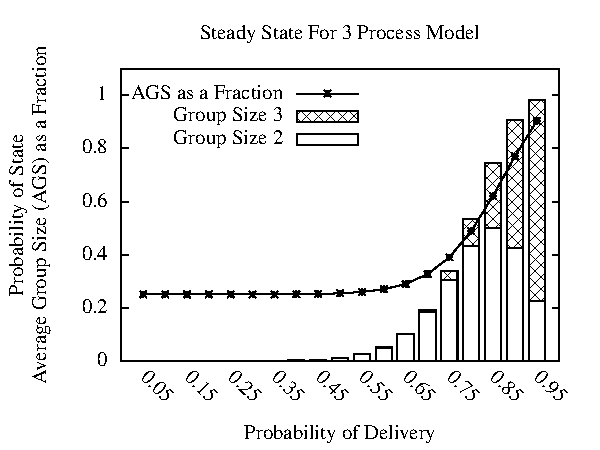
\includegraphics[width=\linewidth]{ss-3process.pdf}
    \caption{Steady state distribution for 3 processes as well as the Average Group Size (AGS) as a fraction of total processes.}
    \label{fig:ss-3process}
\end{figure}

\begin{figure}
    \centering
    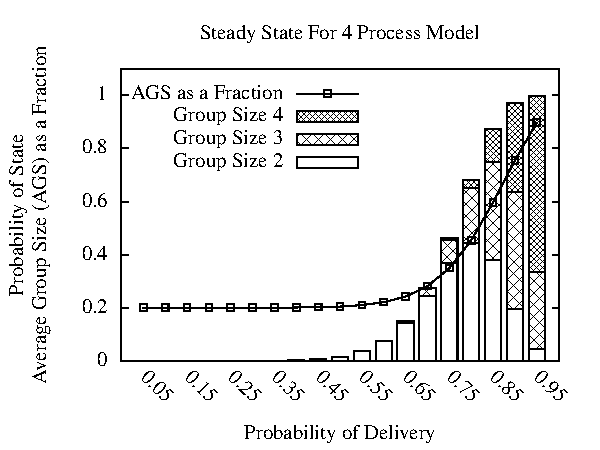
\includegraphics[width=\linewidth]{ss-4process.pdf}
    \caption{Steady state distribution for 4 processes as well as the Average Group Size (AGS) as a fraction of total processes.}
    \label{fig:ss-4process}
\end{figure}

\begin{figure}
    \centering
    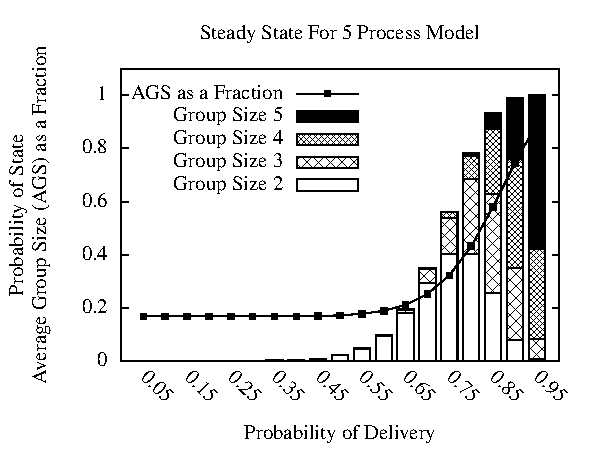
\includegraphics[width=\linewidth]{ss-5process.pdf}
    \caption{Steady state distribution for 5 processes as well as the Average Group Size (AGS) as a fraction of total processes.}
    \label{fig:ss-5process}
\end{figure}

\begin{figure}
    \centering
    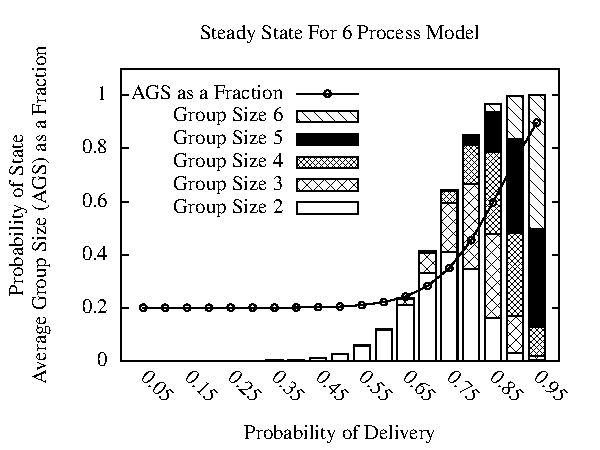
\includegraphics[width=\linewidth]{ss-6process.pdf}
    \caption{Steady state distribution for 6 processes as well as the Average Group Size (AGS) as a fraction of total processes.}
    \label{fig:ss-6process}
\end{figure}

The profile chain can be used to ensure the FREEDM smart grid is able to continue operating despite network issues.
The profile chain can be combined with different message sending strategies to maintain service.
For example, the DGI can change to a slower mode of operation to ensure operation continues normally despite connectivity issues.
By selecting different strategies depending on the message delivery probability the DGI can offer high performance in good network conditions and an acceptable level of service during faults.
The profile chain can be extended to an arbitrary number of processes as shown in Figure \ref{fig:ss-means}.
In Figure \ref{fig:ss-means}, the steady-state of the system is used to compute a weighted average of the group size.
To compare the produced steady states, the weighted average was plotted as a percentage of all processes in the system.
Values in Figure \ref{fig:ss-means}, were plotted using Equation \ref{eq:ss-means}.
Therefore, Figure \ref{fig:ss-means}, shows the average percentage of total processes that will be in the group in a steady-state system.
%Interestingly, the average group size as percentage of the total processes seems to be converging asymptotically, to a fixed value for each plotted probability as the number of processes increases.

\begin{figure}
    \centering
    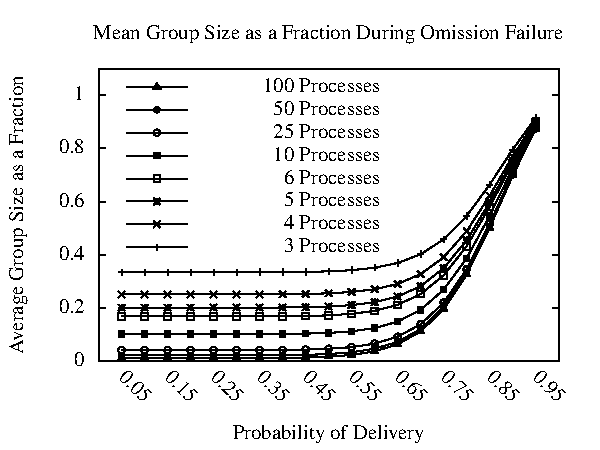
\includegraphics[width=\linewidth]{ss-means.pdf}
    \caption{Average group size as a percentage of all processes in the system for larger systems.}
    \label{fig:ss-means}
\end{figure}

This information can also be used to anticipate faults and mitigate them before they occur.
Modern routers can supply an expected congestion notification as part of the IP header\cite{ECN2}.
When congestion is anticipated, the coordinator can preemptively split the group to reduce congestion.
This is possible because the algorithm's message complexity is $O(n^2)$.
If dropped messages account for an omission rate of even 0.15 from future congestion, performing a coordinated group division can potentially save several rounds of transient states.
Breaking the large groups into smaller sets can drastically reduce the number of messages transmitted and help relieve congestion.
Additionally, the coordinator can design the split to ensure work can continue when the groups are split, by mixing supply and demand processes.
The division can also account for the placement of congested routers for targeted congestion relief.
Furthermore, since the required execution time is a function of group size, the DGI can use the additional execution time within the same real time schedule to use more reliable techniques to deliver messages.

%These techniques allow the DGI to anticipate behavior during a fault and allow it to pre-emptively harden itself against the fault.
